

\documentclass[journal]{IEEEtran}

\usepackage{graphicx}
\usepackage{url}
\usepackage{cite}
\usepackage{authblk}
\usepackage[table,xcdraw]{xcolor}
\usepackage{amssymb}
\usepackage{amsmath}
\begin{document}


\title{Practical Lossless Compression of the Human Movement IMU Signal}
% Compression of Kinematic Data
% Compression of Human Movement Data

\author[1]{David~Chiasson}
\author[1]{Junkai~Xu}
\author[1]{Peter~Shull}
\affil[1]{State Key Laboratory of Mechanical System and Vibration, School of Mechanical Engineering, Shanghai Jiao Tong University}

\maketitle

\begin{abstract}
Real-time human movement inertial measurement unit (IMU) signals are central to many emerging medical and technological applications, yet few techniques have been proposed to process and represent this information modality in an efficient manner. This paper explores techniques for the lossless compression of human movement IMU data. We present several lossless compression methods and compare them with traditional representation formats. Methods are exercised on a public corpus of human movement IMU signals to demonstrate performance. Results show that computationally cheap methods can losslessly compress consumer-grade IMU human movement data with a compression ratio (CR) of 9.6-18.7 depending on movement activity. Furthermore, delta encoding is shown to approach the a posteriori optimal linear compression level. All methods discussed in this study are implemented and released as open source C code using fixed point computation which can be integrated into a variety of computational platforms. These results can be a crucial enabling component of emerging medical and technological applications for the human movement signal.
\end{abstract}

\begin{IEEEkeywords}
kinematic data, human movement, compression, codec
\end{IEEEkeywords}



\section{Introduction}

\IEEEPARstart{M}{any} emerging technological and medical applications rely on real-time human movement IMU signals as a crucial component, including virtual reality\cite{Ahmad2013}, autonomous navigation\cite{Campbell2018}, internet of things\cite{Fernandez-Carames2018}, activity monitoring\cite{Yang2010}\cite{Filippeschi2017}, physical therapy\cite{Patel2012}\cite{Shull2014}, and human performance\cite{Camomilla2018}\cite{GobinathAroganam2019} among others. These applications have been enabled by the recent explosion of cheap inertial based sensors (IMUs) along with mobile computation power to process this data in real time. The human movement IMU signal represents a nascent field of multimedia processing which is starkly under-developed compared to the existing maturity of text, audio, and visual type signal processing methods. This is evidenced by the lack of standards or tools for handling movement data. To enable these emerging applications, efficient and standard methods for representing and processing movement signals are needed. Compression can be a crucial component of the this missing toolset as it improves situations of limited transmission bandwidth and limited storage space.

Compression seeks to represent information in a space efficient manner. This is generally done by exploiting spatio-temporal redundancy, correlation, and smoothness\cite{Sayood2006}. A lossless compression algorithm can be divided into two components, modeling and coding/decoding (Figure \ref{fig:general_compressor})\cite{Nelson1996}. The model incorporates prior understanding of the signal class to be compressed. It estimates a probability mass function which represents the likelihood of occurrence for each possible input symbols. A dynamic model is one which changes its probability estimates after new input symbols are received. The model is sometimes described as a transformation, which refers to some reversible operation which changes the signal into a lower entropy or easier to predict form.  The Coder uses the probability mass function produced by the model to compute a unique variable length encoding for each possible symbol. Short encodings are assigned to likely symbols, and long encodings are assigned to unlikely symbols such that the average length of the compressed signal is minimized. The decompressor uses an identical model to provide the same probability mass function to the decoder which is used to revert each code back into the original symbol. If the model is dynamic, this output is used to update the model for future predictions.


\begin{figure}
  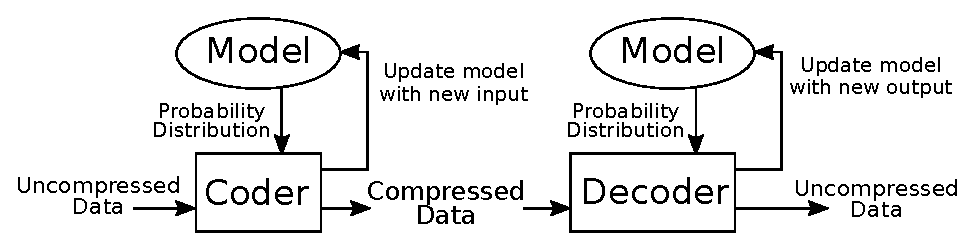
\includegraphics[width=\linewidth]{general_compressor.eps}
  \caption{General compressor and decompressor}
  \label{fig:general_compressor}
\end{figure}

The coding component is well understood. The theoretical limit of coding performance on a signal with a know probability distribution is given by Shannon's noiseless coding theorem\cite{Shannon1948} as first order entropy:

$$H = -\sum_{i} P_ilog_2P_i$$

While Shannon developed several efficient coding techniques, the first optimal technique was developed in 1952 by Huffman\cite{Huffman1952}. While Huffman's technique was proven optimal, it made the assumption that output codes must be an integer number of bits, which prohibited it from reaching Shannon's limit under certain conditions. Arithmetic coding was developed to address this deficiency, showing better performance particularly in high compression situations\cite{Witten1987}. Another technique, Golomb coding and the Rice special case, has experienced significant adoption in industry because of the efficient binary computation, and the ability to encode online without needing a preliminary pass through the data to compute the probability distribution\cite{Golomb1966}\cite{F.Rice1979}. Because of the many efficient and optimal techniques available, some consider coding to be a solved problem\cite{Mahoney2013}.

Modeling on the other hand must be revisited for each new signal class and application. Due to the pigeon hole principal, no algorithm can compress every possible input\cite{Kolmogorov1965}. Each model must make an implicit decision about the class and scope of signals that will be compressed. To the authors' knowledge, no previous work has directly addressed the modeling problem for the human movement IMU signal. This provides the motivation for the current work.


state of modeling in biomed and audio
how it is the same and/or different
what techniques are used


\section{Methods}
This study explores a range of linear predictive models applied to the human movement signal as quantified by 6-axis IMUs. A corpus of representative human movement IMU signals is selected to demonstrate the compression performance of each model. To put the performance in context, several traditional representation formats are selected. The compression performance of these traditional formats provides a lower bound for the performance of a useful compression method. Finally, the optimal linear predictive models are computed numerically utilizing full knowledge of the signals in the corpus. The compression performance of these optimal models provide an upper bound on the performance of our proposed methods.

For this study, the Human Gait Database (HuGaDB)\cite{Chereshnev2018} was selected as a corpus to meaningfully and repeatable demonstrate the performance of various compression methods. HuGaDb is a public dataset of six-axis IMU signals collected from six different body segments (right and left foot, right and left shin, right and left thigh) of 18 healthy subjects performing 12 different movement activities (walking, running, going up and down stairs, sitting, sitting down and standing up, standing, bicycling, going up and down an elevator, and sitting in a car) sampled at 60Hz. This database was selected because it allows the comparison of compression techniques across body segment, subject, and activity.

With the exception of traditional data representation formats, all compression methods in this work will be presented as predictive models. The predictive model will estimate the current sample given past input. The difference between the model prediction and observed sample will be referred to as the residual signal. All compression methods will encode this residual signal using Golomb-Rice coding to produce the final compressed data. Golomb-Rice coding is computationally efficient on binary base computational platforms, and has been shown to approach optimal coding if the input signal is geometrically distributed\cite{Golomb1966}\cite{F.Rice1979}.

\subsection{Proposed Compression Methods}

Several restrictions are placed on the methods considered in this study. First, a viable algorithm must be causal. This is a basic requirement for an algorithm to be implemented in a real-time application. We also chose to only consider algorithms with zero filter delay. Since our sensors operate at a relatively low sampling frequency of 60Hz, a delay of one sample would be 16ms which is significant for modern information networks.

All algorithms considered in this paper are node independent. The model for each signal considers at most the information from the six co-located signals including it's own past input. While it is likely that utilizing inter-node correlation could produce better compression ratios, especially if a human biomechanics model were introduced, such an approach would limit the usefulness of said algorithm to a specific placement of nodes on the body.

Only lossless compression techniques are considered in this study. The reason for this is that lossy compression inherently involves a value judgment about what information is useful and what information is irrelevant. In the absence of a specific application, no justification can be made for discarding any portion of information.

Only lossless algorithms are considered. As discussed in the introduction, a lossy algorithm requires an objective metric for determining how much data loss and of what type is acceptable. Without this metric it is trivial to create a compression algorithm with an infinite compression ratio but which looses all information. [TODO explain more]

In practice, the implementation of a strictly lossless algorithm turns out to be non-trivial. This is because the standard for floating point computation IEEE 754 \cite{Society2008} is not sufficiently stringent to guarantee identical results on various implementations. For example, rounding of results may be slightly different between two computation platforms, or the same computation platform at two points in time. Additionally, a compiler or interpreter which processes the source code for an algorithm implementation will often utilize mathematical properties such as commutativity to optimize computation. This may result in different machines performing floating point operations in a different order which could lead to differing results even if each rounding operation were well defined by IEEE 754. To avoid both of these scenarios and guarantee identical results across diverse computational platforms, all algorithms in this study are implemented using integer operations and fixed-point 16.16 precision. There is significant cost associated with this technical decision. Namely that quantization error is independent of magnitude. This can lead to significant numerical issues for some algorithms.

The following lossless compression techniques are proposed in this study:
\begin{itemize}
  \item \textbf{Delta encoding} Current sample is predicted to be equivalent to the previous sample so that the difference between the two is encoded. If a signal varies slowly with time, this signal will be smaller than the original signal.
  \item \textbf{Linear extrapolation} Current sample is estimated as a linear extrapolation from previous samples. Also known as first order polynomial regression.
  \item \textbf{\boldmath$2^{nd}$ to \boldmath$5^{th}$ order polynomial regression} These techniques assumes that the signal is a polynomial which is estimated from a least squares regression of past samples. This polynomial is then extended to get a prediction of the current sample.
  \item \textbf{Spline extrapolation} A spline is the minimum curvature piece-wise polynomial which connects a set of points. It is commonly used for interpolation, namely computer graphics smoothing. This technique was selected as splines are known to avoid Runge's phenomenon which is witnessed when extrapolating higher order polynomials. Results from the cubic spline with natural boundary conditions are presented in this paper.
\end{itemize}


\subsection{Traditional Representation Formats}
To provide a lower bound for the useful performance of compression techniques, several traditional data representation formats are chosen as reference. In this study, the baseline data format (exhibiting a compression ratio of one) is comma separated value (CSV), a simple text based format which is the de-facto standard for storing sensor information. Performance of each compression technique is evaluated by computing the compression ratio CR relative to CSV via the following formula:
$$CR = \frac{\textrm{size of CSV file}}{\textrm{size of compressed file}}$$

In total, the following three traditional data representation formats were chosen to provide context for our results:

\begin{itemize}
  \item \textbf{CSV} Text based format considered the de facto standard. CSV files are ANSI encoded and formatted to have a constant length sample format to eliminate a source of randomness in our CR computation. Due to this decision, Binary format will have the same CR regardless of data properties. 
  \item \textbf{Binary} The optimal fixed size format. In our corpus, every sample is two bytes. This would be the optimal compression if each sample were an IID random variable uniformly distributed across the sample space.
  \item \textbf{ZIP compression of CSV} ZIP is a general purpose file compression format integrated into all major computer systems. ZIP was executed using the DEFLATE method \cite{Deutsch1996} and a compression level of 6.
\end{itemize}

\subsection{Optimal Linear Compression}

To complete the context for our proposed compression methods and provide an upper limit on compression performance, we numerically compute the optimal linear predictive model for our data. To do so, we will formulate our model as an auto-regressive process of order $p$ and define the prediction error or residual signal as:

\begin{equation}
e[n] = x[n] - \sum_{k=1}^{p}a_{k}x[n-k]
\label{eq:error}
\end{equation}
where $a_k$ is the linear contribution of sample $k$ in the past to our current prediction. Equation \eqref{eq:error} can expressed be in concise matrix notation as: 

$$\mathbf{e} = \mathbf{x} - \mathbf{Xa}$$

For our application, we are interested in the residual signal $\mathbf{e}$ which can be encoded into the minimum number of bits. To compute this, we consider the effect of Rice-Golomb coding on our residual signal. A Rice-Golomb encoding of order $m \in \mathbb{N}_0$, first splits each residual $e[n]$ into a quotient and remainder portion:

$$ q[n] = \lfloor \frac{e[n]}{2^m} \rfloor\quad \textrm{and} \quad r[n] = e[n] - q[n] * 2^m  $$

The remainder $r[n]$ is truncated binary encoded at a fixed size of $m$ bytes, while the quotient $q[n]$ is unary encoded, requiring $q[n] + 1$ bits. The size in bits of each Rice-Golomb encoded element of the residual signal is thus:

$$ m + \lfloor\frac{e[n]}{2^m}\rfloor + 1$$

If we relax our rounding operation, the size of each element can be approximated as a affine function of $e[n]$. The total compressed size for a signal of length $l$ has an approximate size:
 $$l+lm+ 2^{-m}\sum_{n=0}^l e[n]$$
 Minimizing this value with $l$-1 normalization is equivalent to the optimization problem:
 
\begin{equation}
\begin{aligned}
& \underset{\mathbf{a}}{\text{minimize}}
& & \left\Vert \mathbf{x}-\mathbf{Xa} \right\Vert_1 + \lambda\left\Vert \mathbf{a} \right\Vert_1
\label{eq:optimize}
\end{aligned}
\end{equation}

The key takeaway from this result, is that compression is proportional to the total \textit{absolute prediction error} of the model, and not the \textit{squared error}. $l$-1 normalization is used since it encourages sparsity in the model. Sparsity is desirable in this application as it reduces quantization error of the model coefficients and reduces the fixed point arithmetic error during execution. Both of these sources of error are significant when performing fixed point arithmetic. Since this problem is convex, it can readily be solved with a variety of numerical solvers. For this study, python bindings for the Splitting Conic Solver were used\cite{ocpb:16}\cite{scs}\cite{cvxpy}.

If problem \eqref{eq:optimize} is solved considering past history of each stream, then the model for each axis of accelerometer and gyroscope can be computed independently. This model will be referred to as the optimal auto-regressive model (AR). However, if we also take into account the past history of other axes and sensors, then the model can account for any cross-correlation which may result from the interrelated nature of rotation and orientation information. The residual signal using this expanded model for stream $i$ is:

\begin{equation}
e_i[n] = x_i[n] - \sum_{j=1}^{s}\sum_{k=1}^{p}a_{i,j,k}x_j[n-k]
\label{eq:error}
\end{equation}

where $a_{i,j,k}$ is now the linear contribution of the sample $k$ in the past of stream $j$ to our current prediction of stream $i$. Solving problem \eqref{eq:optimize} with this expanded system will be referred to as the optimal multivariate autoregressive model (MVAR).

\subsection{Implementation}

This study focuses on highly practical approaches which can be used in modern applications. To demonstrate this, all compression techniques have been implemented and released as open-source C code using fixed point computations. The hope of the authors is that this code can be a starting point for academic or industry developers implementing some human movement application on diverse computational platforms.

To show algorithm performance in a realistic scenario, as well as to provide tools of benefit to the community, the algorithms in this study were implemented in the C programming language and released as open-source code found at \url{https://github.com/dchiasson/kinetic_codec}.[TODO: move to results?] The choice of programming language as well as the restriction to integer arithmetic allow this code to be easily incorporated into programs executing on either a personal computer or embedded computation platforms, even those without a floating-point unit.

\section{Results}
[TODO: consider computation time?]
All proposed compression methods outperformed traditional methods in size efficiency (Table \ref{table:all_stats}). Delta encoding achieved the highest compression of the polynomial regression methods (CR=12.75), and each higher degree polynomial performed progressively worse with 5th degree polynomial at the bottom (CR=11.25). The CR of delta encoding approached and occasionally exceeded that of the optimal AR and MVAR model.

Low movement activities such as sitting and standing were compressed much more than high movement activities such as running (Fig:\ref{fig:movements}). Body segments showed little variation in CR although thigh locations showing slightly higher compression (Fig:\ref{fig:segments}).

\begin{figure}

  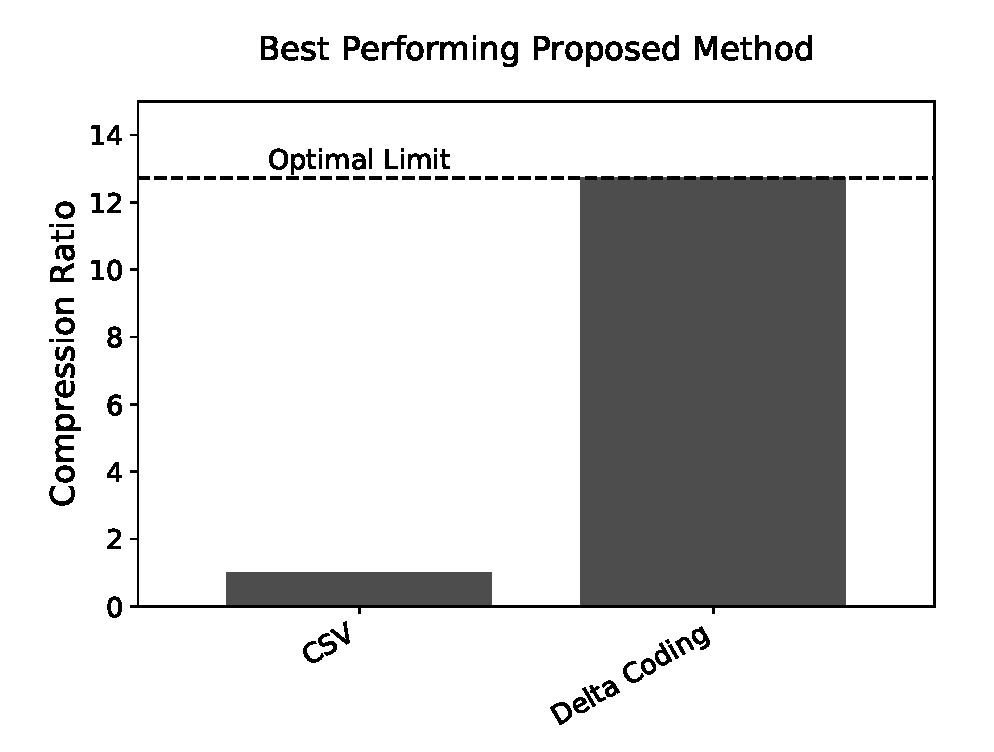
\includegraphics[width=\linewidth]{diff.eps}
  \caption{Compression ratio (original size / compressed size) of delta encoding compared with traditional CSV. Delta encoding approaches the optimal auto-regressive compression level.}
  \label{fig:main_results}
  
\end{figure}
\begin{figure}

  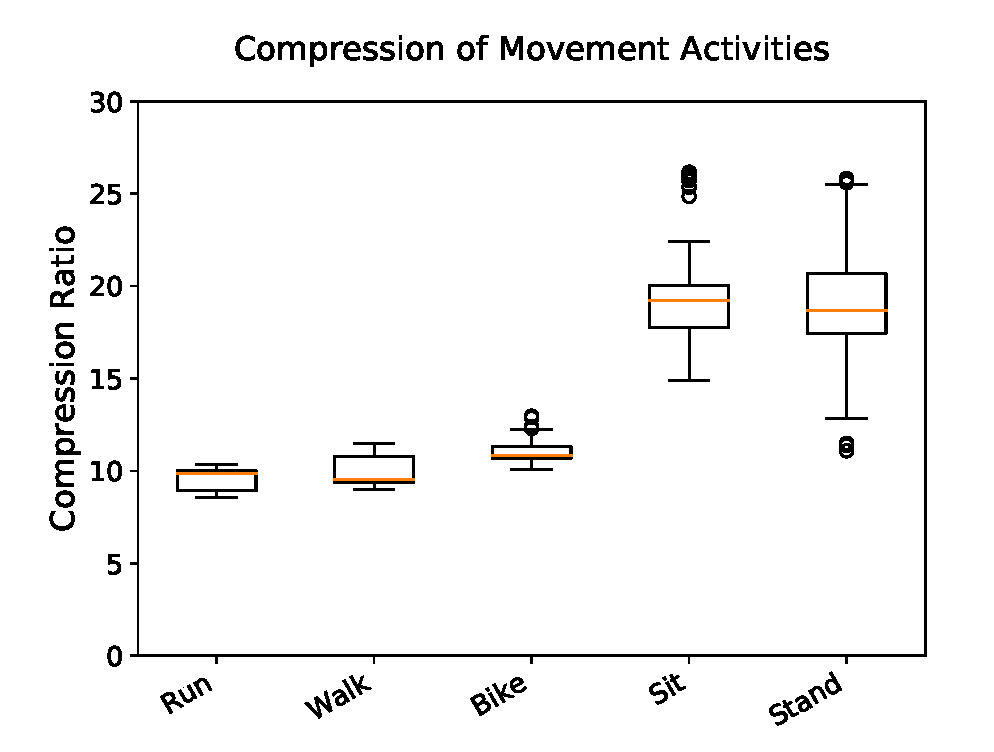
\includegraphics[width=\linewidth]{movement.eps}
  \caption{[Compression ratio (original size / compressed size) of each movement activity using delta encoding. Activities with greater movement intensity experience significantly less compression.}
  \label{fig:movements}
  
\end{figure}
\begin{figure}

  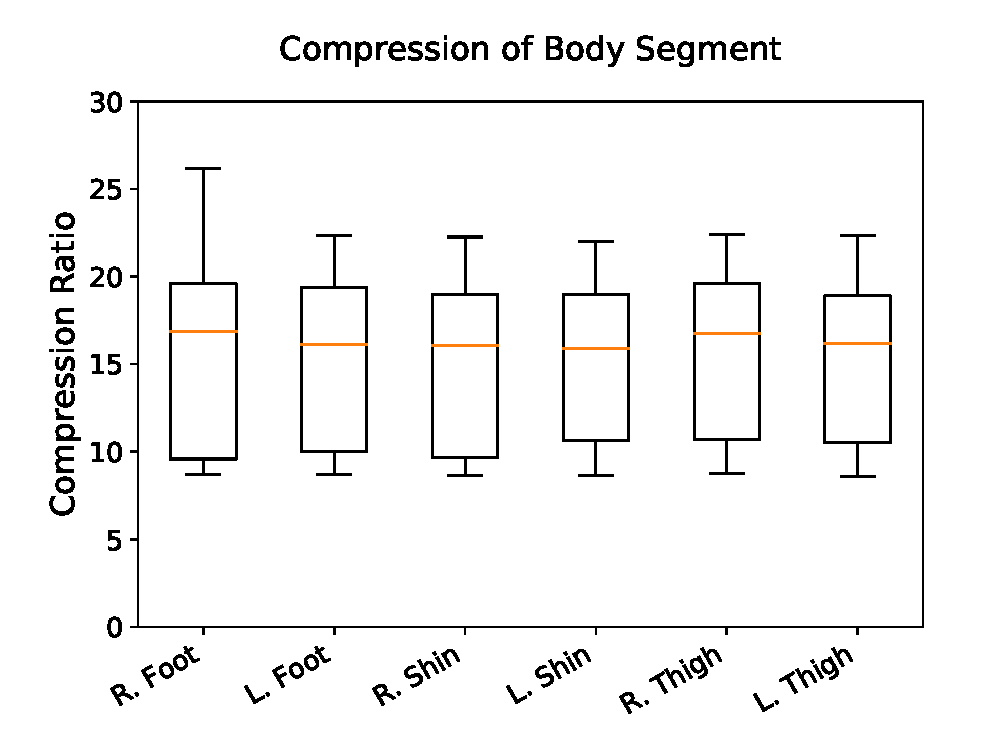
\includegraphics[width=\linewidth]{segment.eps}
  \caption{Compression ratio (original size / compressed size) of each body segment using delta encoding. Body segment has little effect on compression ratio.}
  \label{fig:segments}
  
\end{figure}

%http://www.tablesgenerator.com/latex_tables
%http://calc2latex.sourceforge.net/

\begin{table*}[htbp]
\caption{Compression ratios for all methods across movement activity and body segment}
\label{table:all_stats}
\resizebox{\textwidth}{!}{%
\begin{tabular}{|l|r|r|r|r|r|r|r|r|r|r|r|r|}

\hline
 & \multicolumn{1}{l|}{\textbf{}} & \multicolumn{ 5}{c|}{\textbf{Activity}} & \multicolumn{ 6}{c|}{\textbf{Body Segment}} \\ \hline
 & \multicolumn{1}{l|}{\textbf{}} & \multicolumn{1}{l|}{\textbf{}} & \multicolumn{1}{l|}{\textbf{}} & \multicolumn{1}{l|}{\textbf{}} & \multicolumn{1}{l|}{\textbf{}} & \multicolumn{1}{l|}{\textbf{}} & \multicolumn{ 2}{c|}{\textbf{Foot}} & \multicolumn{ 2}{c|}{\textbf{Shin}} & \multicolumn{ 2}{c|}{\textbf{Thigh}} \\ \hline
 & \multicolumn{1}{l|}{\textbf{All}} & \multicolumn{1}{l|}{\textbf{Walk}} & \multicolumn{1}{l|}{\textbf{Run}} & \multicolumn{1}{l|}{\textbf{Sit}} & \multicolumn{1}{l|}{\textbf{Stand}} & \multicolumn{1}{l|}{\textbf{Bike}} & \multicolumn{1}{l|}{\textbf{R}} & \multicolumn{1}{l|}{\textbf{L}} & \multicolumn{1}{l|}{\textbf{R}} & \multicolumn{1}{l|}{\textbf{L}} & \multicolumn{1}{l|}{\textbf{R}} & \multicolumn{1}{l|}{\textbf{L}} \\ \hline
\textbf{CSV} & 1.00 & 1.00 & 1.00 & 1.00 & 1.00 & 1.00 & 1.00 & 1.00 & 1.00 & 1.00 & 1.00 & 1.00 \\ \hline
\textbf{ZIP} & 3.97 & 3.06 & 3.26 & 6.07 & 6.18 & 3.09 & 3.99 & 4.10 & 3.95 & 3.98 & 3.98 & 3.93 \\ \hline
\textbf{Binary} & 8.32 & 8.32 & 8.32 & 8.32 & 8.32 & 8.32 & 8.32 & 8.32 & 8.32 & 8.32 & 8.32 & 8.32 \\ \hline
\textbf{Spline} & 12.20 & 9.63 & 9.23 & 16.61 & 17.24 & 10.74 & 12.04 & 11.99 & 11.98 & 12.12 & 12.60 & 12.48 \\ \hline
\textbf{5th deg. poly.} & 11.25 & 8.92 & 8.59 & 15.28 & 15.78 & 9.87 & 11.24 & 11.16 & 11.10 & 11.20 & 11.49 & 11.34 \\ \hline
\textbf{4th deg. poly.} & 11.57 & 9.09 & 8.73 & 15.93 & 16.39 & 10.15 & 11.54 & 11.47 & 11.42 & 11.54 & 11.81 & 11.65 \\ \hline
\textbf{3rd deg. poly.} & 11.80 & 9.22 & 8.84 & 16.44 & 16.80 & 10.30 & 11.74 & 11.67 & 11.66 & 11.78 & 12.05 & 11.88 \\ \hline
\textbf{2nd deg. poly.} & 12.00 & 9.35 & 8.97 & 16.77 & 17.29 & 10.44 & 11.95 & 11.87 & 11.85 & 12.00 & 12.25 & 12.07 \\ \hline
\textbf{Linear} & 12.22 & 9.52 & 9.11 & 17.19 & 17.81 & 10.52 & 12.21 & 12.11 & 12.07 & 12.20 & 12.45 & 12.26 \\ \hline
\textbf{Delta} & 12.75 & 9.95 & 9.52 & 17.87 & 18.69 & 10.96 & 12.68 & 12.61 & 12.54 & 12.71 & 13.07 & 12.87 \\ \hline
\textbf{Optimal AR} & 12.73 & 9.93 & 9.54 & 17.87 & 18.76 & 11.12 & 12.61 & 12.55 & 12.48 & 12.68 & 13.12 & 12.92 \\ \hline
\textbf{Optimal MVAR} & 12.70 & 9.93 & 9.56 & 17.83 & 18.67 & 11.12 & 12.50 & 12.26 & 12.34 & 12.60 & 12.90 & 12.70 \\ \hline


\end{tabular}%
}%

\end{table*}



\section{Discussion}

These results show that even simple techniques result in a significant compression over the traditional encoding of CSV. If bandwidth or storage space is a concern in a human movement IMU application, then using any of the proposed methods would be an improvement.

This increasingly poor performance by higher order polynomials is likely because higher degree polynomial predictors suffer from poor white noise attenuation \cite{Tanskanen2000} causing an effect known as Runge's phenomenon.

Delta encoding performed surprisingly well, even exceeding that of the optimal linear models on several occasions. In theory, the optimal linear models should perform as well or better than delta encoding, since delta encoding is within the class of models that were optimized over in equation \eqref{eq:optimize} . The occasional inferior performance of the optimal linear models can be attributed to quantization error of the model coefficients and increased fixed point error from computational complexity. This explanation is supported by the observation that the cross-correlation model, which has a more complex model, often underperforms relative to the auto-regressive model while the opposite would be true in the absence of numeric error. Investigation of the optimal models' coefficients showed that they were similar to those of delta encoding.

The compression level achieved on each movement activity varied greatly, and appears roughly correlated with the intensity of movement involved in that activity (Fig:\ref{fig:movements}) . This matches our expectations as higher intensity of movement will intuitively have more information content. The compression of body segment information (Fig:\ref{fig:segments}) showed very minor variations save for slightly more compression of the thigh information. Intuitively, the thigh will experience less intense movement during most human movement. We can also observe minor differences between the compression of right and left body segments of the same type. Since the movement activities explored in this study are symmetric, these differences in compression are likely indicative of noise and bias differences between hardware sensors.

The similar performance of the MVAR optimal model and the AR optimal model does not support the expected redundancy between accelerometer and gyroscope information. If such a linear correlation exists, it is too small to be usable in this practical application. This study does not preclude the possibility of a non-linear model to successfully exploit such a relationship.

[TODO] Why is delta so good? it is just as good in other realms. Computational complexity of delta

Four sources of error for optimal: quantization, computational, convergance error, model assumption

The compression ratios presented in this paper are intended to demonstrate the relative difference between compression techniques and may not be representative of the absolute CR experienced in other applications. There are many other factors which can affect the compression ratio which are not explored in this paper. Namely, sensor differences of precision, noise, bias, and sampling rate are expected to have a large impact on the CR achieved. That being said, low-cost consumer grade IMUs were used for this study at a low sampling rate, and the authors would expect many applications to experience significantly higher compression than presented here if higher sampling rate or higher quality sensors are used.

The corpus chosen for demonstrating performance in this work allowed us to explore the effect of movement activity and body segment on compression. However, it could be improved for this purpose by including diverse hardware and higher sampling rates which would be more representative of applications.

Future work includes:

dynamic or non-linear models (utilize rotation)
arithmetic coding
dynamic K detection
data packet drop recovery
lossy techniques (define a standard for acceptable loss)
inter sensor correlation
magnetometer
standardized data format

\section{Conclusion}
This work explores methods for the compression of human movement IMU signal. Greater compression will improve data transmission throughput and storage efficiency, potentially enabling new technology applications which were previously infeasible. For the corpus selected, delta encoding provided near-optimal linear compression (factor of 9.6-18.7 times) with very low computational cost.

\section*{Acknowledgment}
This work was supported by the National Natural Science
Foundation of China (51875347).

\bibliography{mendeley_citations,other_citations}{}
\bibliographystyle{plain}
%TODO: Make sure bib style is correct!
%\bibitem{IEEEhowto:kopka}

\clearpage
\section*{Scratch Section}
TODO: rewrite paragraphs below, maybe drop or move to method

The goal of the model is to produce an accurate PMF with minimum entropy. Intuitively this means that compression is higher the more "sure" the model is about some occurrences over other ones. If an optimal encoder is used, the compression ratio can be regarded as a quantitative measurement of the model's understanding of the underlying signal. Because of this, we expect the performance of various signal models to give us insight into the content of the kinematic signal.

The same coder and decoder is employed by all compression techniques explored in this work, and techniques are thus identified by the model used. Models are presented as predictive algorithms. Using this paradigm, the residual is the difference between each input symbol and what the model predicted the symbol to be. The compressed size is the first order entropy of the residual signal.


Consider deleting below:

TODO: why do we assume our signal is geometrically distributed about the mean!?
TODO: relationship for natural signals of residual signal and compression ratio

In this work, the maximum likelihood occurrence according to the model will be referred to as the prediction. The difference between the prediction and the actual sample will be referred to as the residual. For practical implementation, it is advantageous to convert the original signal into the residual signal before coding so that the coder can be computationally optimized to compute encodings for zero mean random variables (or same distribution? not recalculating ).

Define stream? node? anything else?

Linearized rotating gravity - A Newtonian physics based model in which a constant magnitude acceleration vector rotates according to gyroscope readings.

Finally, this study only explores linear models. Why is that?

 In the context of compression, complex or numerically unstable algorithms may produce compression ratios which underestimate their understanding of the underlying signal since their implementation is not equivalent to their mathematical derivation.

TODO: handle negatives in optimal filter derivation!

TODO: quantify statistical significance

Tables of detailed results k, order: total, accel/gryo, activity, segment, subject 

TODO: Discussion of cross stream FIR coefficients, pole zero plots, precision effect

TODO: Medical names for body parts?

TODO: can I prove that the optimal IIR linear filter cannot exceed that of the optimal FIR linear filter?

TODO: add algorithm execution time

TODO: Too many synonyms? [signal, data, file] [encoding, algorithm, model, technique, representation, compression, method] [kinematic, human movement]
TODO: audio compression comparison of methods and performance
TODO: what verb tense where?
TODO: demonstrate long implementation of compression technique to show that error is from quantization and fixed point error
TODO: re clarify hypothesis, discuss what was verified
TODO[change the name of the repo, clean up docs, and release]. 
TODO[reformat table]
TODO: can I reference solved problem Mahoney2013?
[TODO remove?]  We hypothesized that compression ratios would be comparable to those achieved in lossless audio compression. We also hypothesized that the best performing method will utilize some cross axis correlation and be informed by physics based models.
[TODO] find better pidgeon hole citation


\end{document}
